%%%%%%%%%%%%%%%%%%%%%%%%%%%%%%%%%%%%%%%%%
% LaTeX Template
% http://www.LaTeXTemplates.com
%
% Original author:
% Linux and Unix Users Group at Virginia Tech Wiki 
% (https://vtluug.org/wiki/Example_LaTeX_chem_lab_report)
%
% License:
% CC BY-NC-SA 3.0 (http://creativecommons.org/licenses/by-nc-sa/3.0/)
%
%%%%%%%%%%%%%%%%%%%%%%%%%%%%%%%%%%%%%%%%%

%----------------------------------------------------------------------------------------
%	PACKAGES AND DOCUMENT CONFIGURATIONS
%----------------------------------------------------------------------------------------

\documentclass[12pt]{article}
\usepackage{geometry} % Pour passer au format A4
\geometry{hmargin=1cm, vmargin=0.5cm} % 

\usepackage{graphicx} % Required for including pictures
\usepackage{float} % 

%Français
\usepackage[T1]{fontenc} 
\usepackage[english,francais]{babel}
\usepackage[utf8]{inputenc}
\usepackage{eurosym}
\usepackage{lmodern}
\usepackage{url}
\usepackage{multicol}
\usepackage{multido}

%Maths
\usepackage{amsmath,amsfonts,amssymb,amsthm}
%\usepackage[linesnumbered, ruled, vlined]{algorithm2e}
%\SetAlFnt{\small\sffamily}

%Autres
\linespread{1} % Line spacing
\setlength\parindent{0pt} % Removes all indentation from paragraphs

\newcommand{\horrule}[1]{\rule{\linewidth}{#1}} % Create horizontal rule 
\renewcommand{\labelenumi}{\alph{enumi}.} % 

\newcommand{\Pointille}[1][3]{\multido{}{#1}{    \makebox[\linewidth]{\dotfill}\\[\parskip]}}

\pagestyle{empty}
%----------------------------------------------------------------------------------------
%	DOCUMENT INFORMATION
%----------------------------------------------------------------------------------------
\begin{document}
\setlength{\columnseprule}{1pt}

%\maketitle % Insert the title, author and date

\textbf{Nom(s), Prénom(s) :}

\begin{center}
  \textit{Le courage est le juste milieu entre la peur et l'audace}\\ \textbf{- Aristote -}
\end{center}


\textbf{Exercice 1}

Ici $t$ (en secondes) désigne le temps mis pour parcourir la distance $d$ (en mètres) à la vitesse moyenne $v$ (en m/s).

\begin{center}
\begin{tabular}{|p{1cm}|p{2cm}|p{2cm}|p{2cm}|p{2cm}|p{2cm}|}
  \hline
   d $\phantom{\dfrac{a}{b}}$ & 250 & 180 & 700 & \\
  \hline
   v $\phantom{\dfrac{a}{b}}$ &     &     &  15 &  5 \\
  \hline
   t $\phantom{\dfrac{a}{b}}$ &   5 &  20 &     &   35\\
  \hline
\end{tabular}
\end{center}

\horrule{1px}

\textbf{Pour les exercices 2 et 3, il est demandé de laisser apparaître une trace des calculs et de répondre à la question par une phrase.}

\begin{multicols}{2}

  \textbf{Exercice 2}\\
Antoine a parcouru 104 mètres en 4 secondes sur une route départementale.\\
A-t-il dépassé la vitesse limite de 90 km / h ?
  \Pointille[9]

\end{multicols}

\horrule{1px}

\begin{multicols}{2}
\textbf{Exercice 3}\\
Max a parcourut 150 km à la vitesse moyenne de 130 km /h puis 125 km à 100 km /h.\\
Il prétend qu'il a réalisé 110 km / h de moyenne pour effectuer son parcours. Qu'en pensez-vous ?
  \Pointille[9]

\end{multicols}

\horrule{1px}

\begin{multicols}{3}

  \textbf{Exercice 4}\\
  \textbf{Les triangles suivants sont-ils rectangles ?} \textit{Justifier.}
  
  \begin{figure}[H]
    \centering
    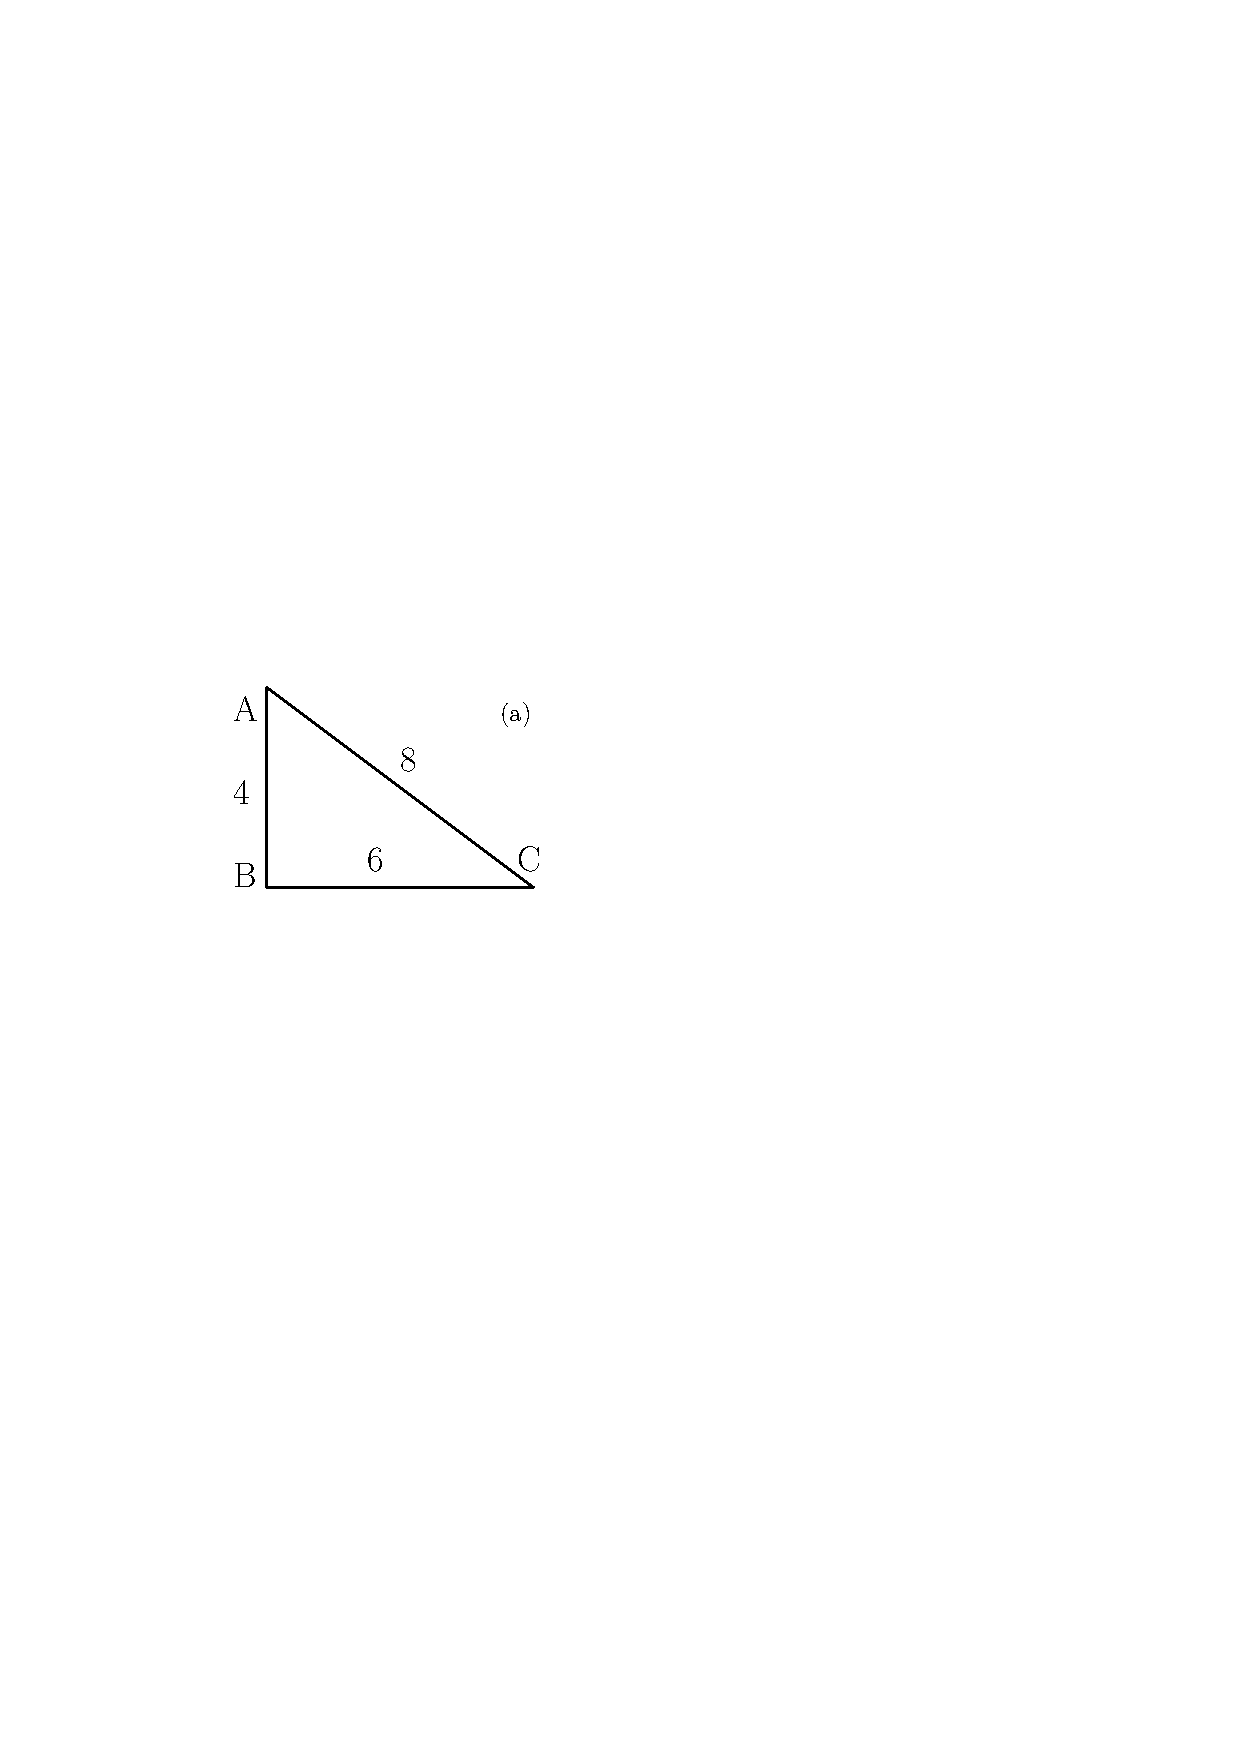
\includegraphics[width=0.7\linewidth]{sources/1/exo2-tri-1.pdf}
  \end{figure}

  \begin{figure}[H]
    \centering
    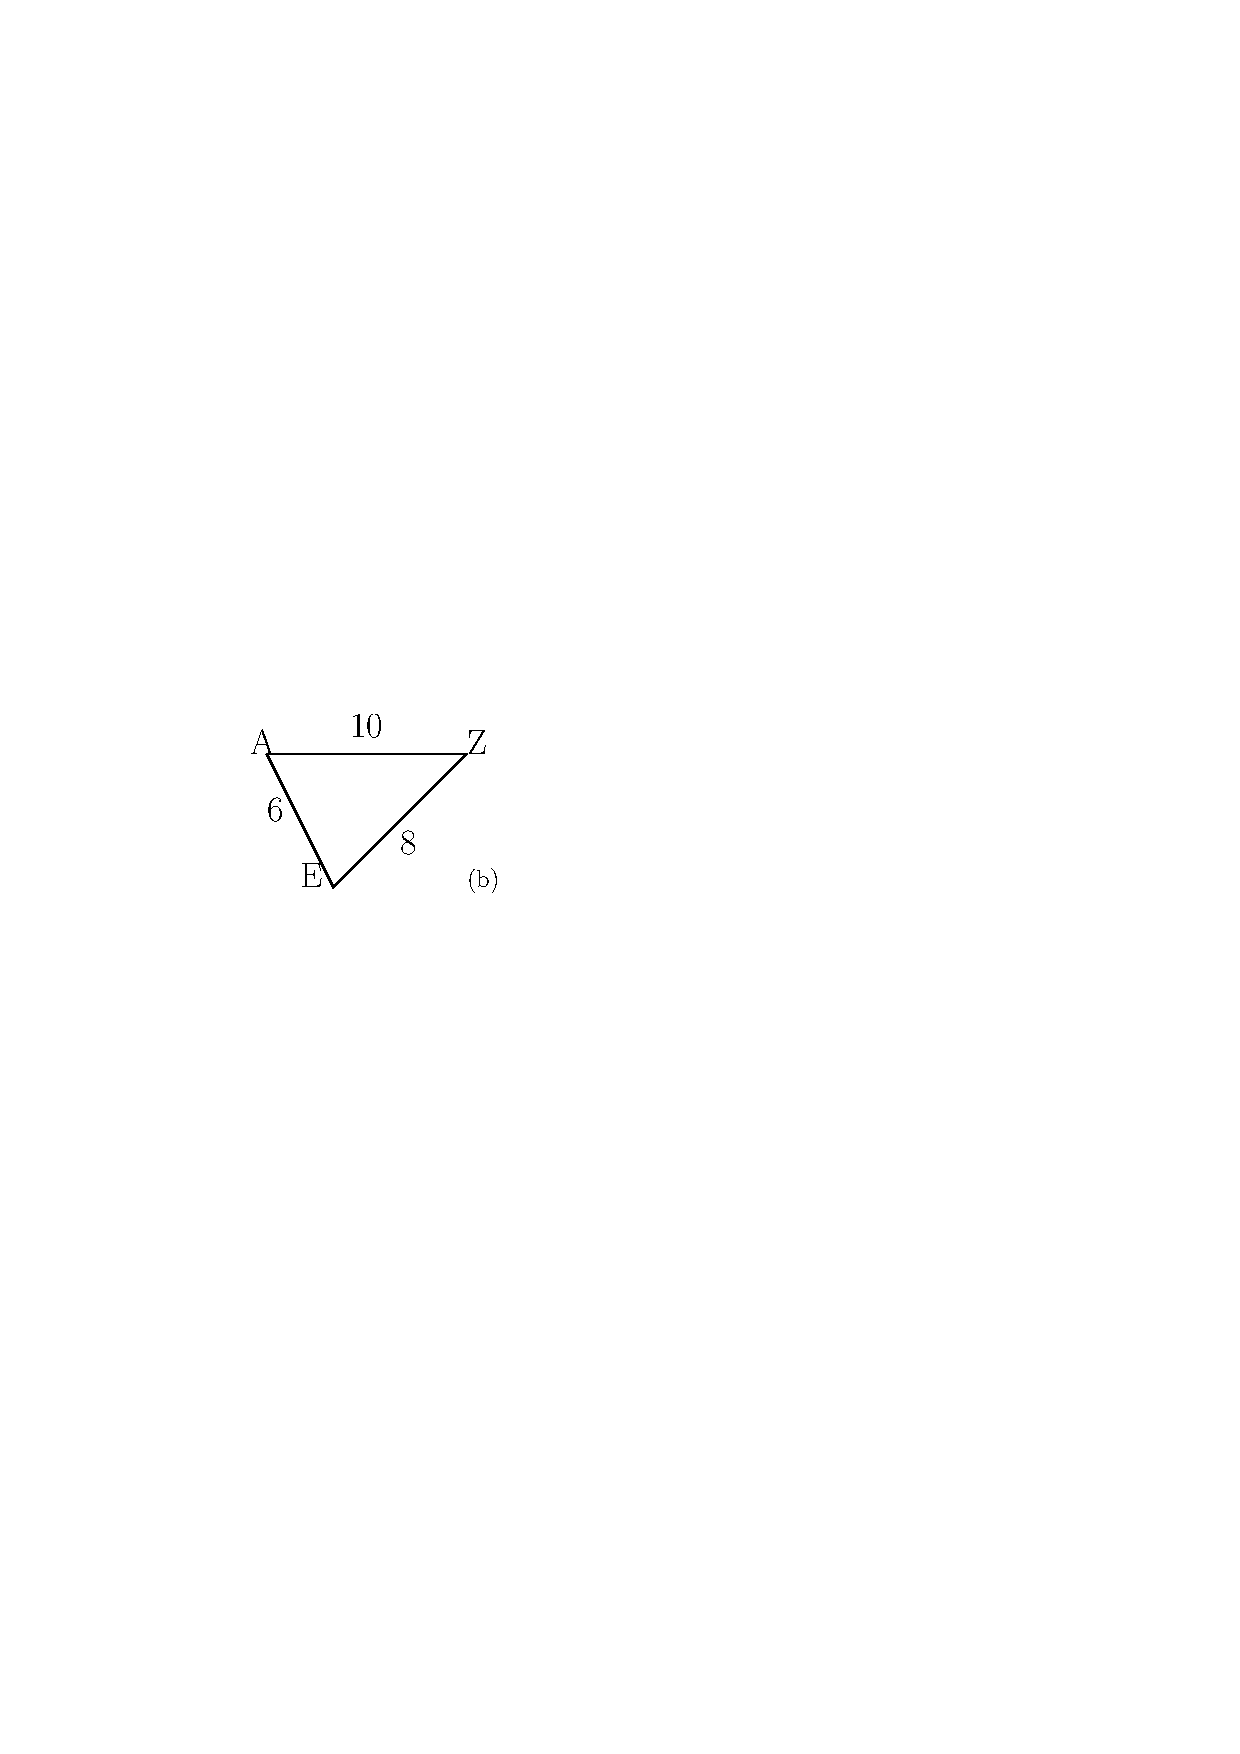
\includegraphics[width=0.7\linewidth]{sources/1/exo2-tri-2.pdf}
  \end{figure}
\end{multicols}

\begin{multicols}{2}
\begin{enumerate}
\item[a.] \Pointille[6]
\item[b.] \Pointille[6]
\end{enumerate}
\end{multicols}
\end{document}
